%GiG
\documentclass{beamer} 
\usetheme{Copenhagen}
\setbeamertemplate{navigation symbols}{}
\setbeamertemplate{headline}{}
\DeclareMathOperator*{\argmax}{arg\,max}

\usepackage{hyperref}
\definecolor{azure}{rgb}{0.0, 0.5, 1.0}
%\newcommand{\tblue}[1]{\textcolor{blue}{#1}}
\newcommand{\tblue}[1]{{\Large {\textcolor{azure}{#1}}}}
\newcommand{\hred}[1]{{\textcolor{red}{#1}}}

\title[Saravanan Thirumuruganathan] 
{Lecture 2: Divide\&Conquer Paradigm, Merge sort and Quicksort}

\author[CSE 5311] 
{Instructor: Saravanan Thirumuruganathan}

\date[] 

\begin{document}

\begin{frame}
  \titlepage
\end{frame}

%\begin{frame}{Outline}
%  \tableofcontents
%  % You might wish to add the option [pausesections]
%\end{frame}

\section{Outline}

\begin{frame}
\frametitle {Outline}
\begin{enumerate}
\item Divide and Conquer
\item Merge sort
\item Quick sort
\end{enumerate}
\end{frame}

\begin{frame}{In-Class Quizzes}
\begin{itemize}
\item {\Large {\bf URL:}} {\LARGE \bf \url{http://m.socrative.com/}} 
\item {\Large {\bf Room Name:} {\LARGE \bf 4f2bb99e}}
\end{itemize}
\end{frame}

\section{Divide and Conquer Paradigm}

\begin{frame}{Divide And Conquer Paradigm}
\begin{itemize}
\item D\&C is a popular algorithmic technique
\item Lots of applications
\item Consists of three steps:
\begin{enumerate}
    \item {\bf Divide} the problem into a number of sub-problems
    \item {\bf Conquer} the sub-problems by solving them {\em recursively}
    \item {\bf Combine} the solutions to sub-problems into solution for original problem 
\end{enumerate}
\end{itemize}
\end{frame}


\begin{frame}{Divide And Conquer Paradigm}

\tblue{When can you use it?}
\begin{itemize}
\item The sub-problems are easier to solve than original problem
\item The number of sub-problems is {\bf small}
\item Solution to original problem can be obtained easily, once the sub-problems are solved
\end{itemize}
\end{frame}


\begin{frame}{Recursion and Recurrences}
\begin{itemize}
\item Typically, D\&C algorithms use {\bf recursion} as it makes coding simpler
\item Non-recursive variants can be designed, but are often slower
\item If all sub-problems are of equal size, can be analyzed by the recurrence equation 
$$ T(n) = a T(\frac{n}{b}) + D(n) + C(n)$$
\item $a$: number of sub-problems to solve 
\item $b$: how fast the problem size shrinks
\item $D(n)$: time complexity for the divide step
\item $C(n)$: time complexity for the combine step
\end{itemize}
\end{frame}

\begin{frame}{D\&C Approach to Sorting}

\tblue{How to use D\&C in Sorting?}
\begin{itemize}
\item Partition the array into sub-groups
\item Sort each sub-group recursively
\item Combine sorted sub-groups if needed
\end{itemize}
\end{frame}

\section{Merge Sort}
\begin{frame}{Why study Merge Sort?}
\begin{itemize}
\item One of the simplest and efficient sorting algorithms
\item Time complexity is $\Theta(n \log n)$ (vast improvement over Bubble, Selection and Insertion sorts)
\item Transparent application of D\&C paradigm
\item Good showcase for time complexity analysis
\end{itemize}
\end{frame}


\begin{frame}{Merge Sort}

\tblue{High Level Idea :}
\begin{itemize}
\item Divide the array into two {\bf equal} partitions - $L$ and $R$ 
\begin{itemize}
    \item If not divisible by 1, $L$ has $\lfloor \frac{n}{2} \rfloor$ elements and $R$ has $\lceil \frac{n}{2} \rceil$
\end{itemize}
\item Sort left partition $L$ recursively
\item Sort right partition $R$ recursively
\item Merge the two sorted partitions into the output array
\end{itemize}
\end{frame}


\begin{frame}[fragile]{Merge Sort Pseudocode}

\tblue{Pseudocode:}
\begin{verbatim}
MergeSort(A, p, r):
    if p < r:
        q = (p+r)/2
        Mergesort(A, p , q)
        Mergesort(A, q+1, r)
        Merge(A, p, q, r)
\end{verbatim}
\end{frame}


\begin{frame}{Merge Sort - Divide\footnote{\url{http://web.stanford.edu/class/cs161/slides/0623_mergesort.pdf}}}
\begin{center}
    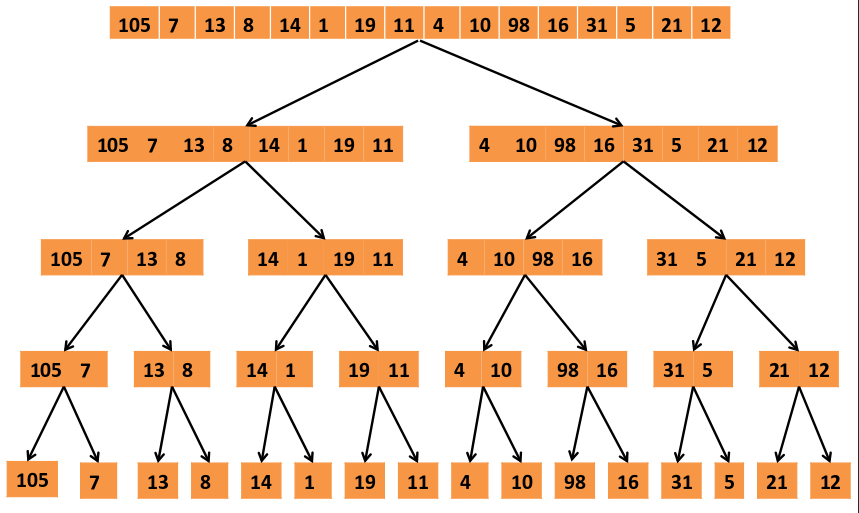
\includegraphics[scale=0.38]{mergeSortRecursion.png}
\end{center}
\end{frame}


\begin{frame}{Merge Sort - Combine\footnote{\url{http://web.stanford.edu/class/cs161/slides/0623_mergesort.pdf}}}
\begin{center}
    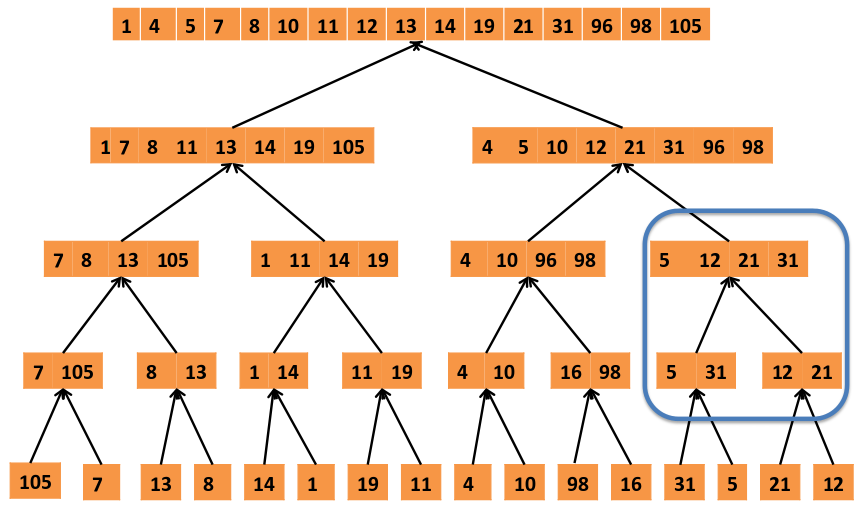
\includegraphics[scale=0.36]{mergeSortMerge.png}
\end{center}
\end{frame}


\begin{frame}{Merging Two Sorted Lists\footnote{\url{http://web.stanford.edu/class/cs161/slides/0623_mergesort.pdf}}}
\begin{center}
    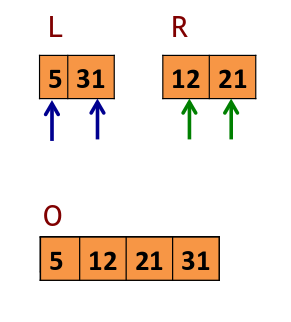
\includegraphics[scale=0.5]{mergeListExample.png}
\end{center}
\end{frame}


\begin{frame}{Merging Two Sorted Lists}
\begin{center}
    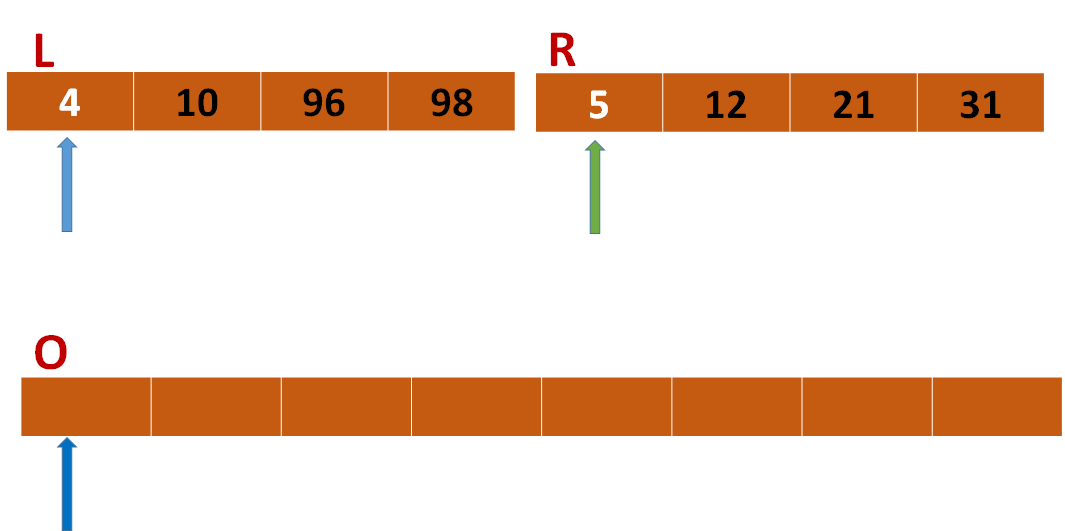
\includegraphics[scale=0.4]{mergeStep1.png}
\end{center}
\end{frame}




\begin{frame}{Merging Two Sorted Lists}
\begin{center}
    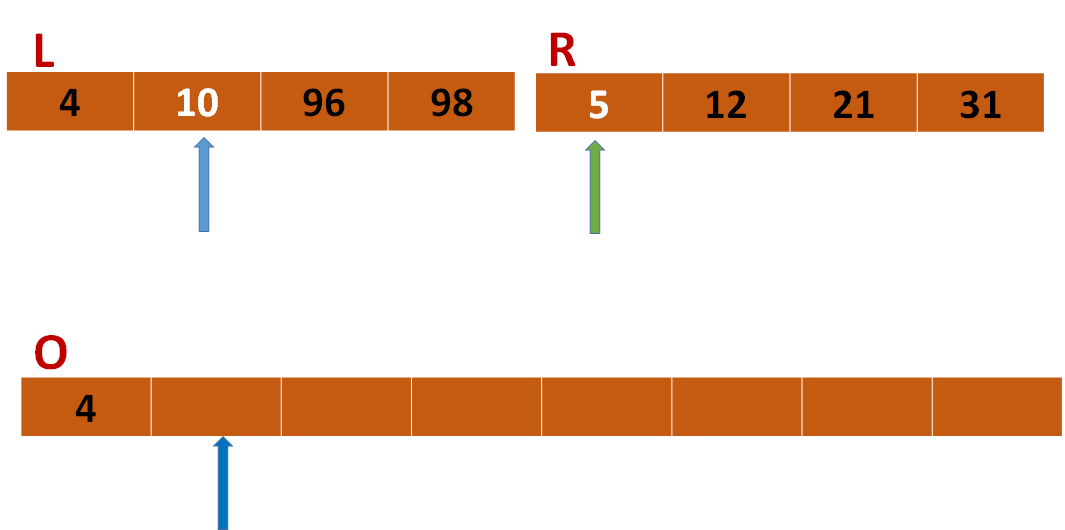
\includegraphics[scale=0.4]{mergeStep2.png}
\end{center}
\end{frame}




\begin{frame}{Merging Two Sorted Lists}
\begin{center}
    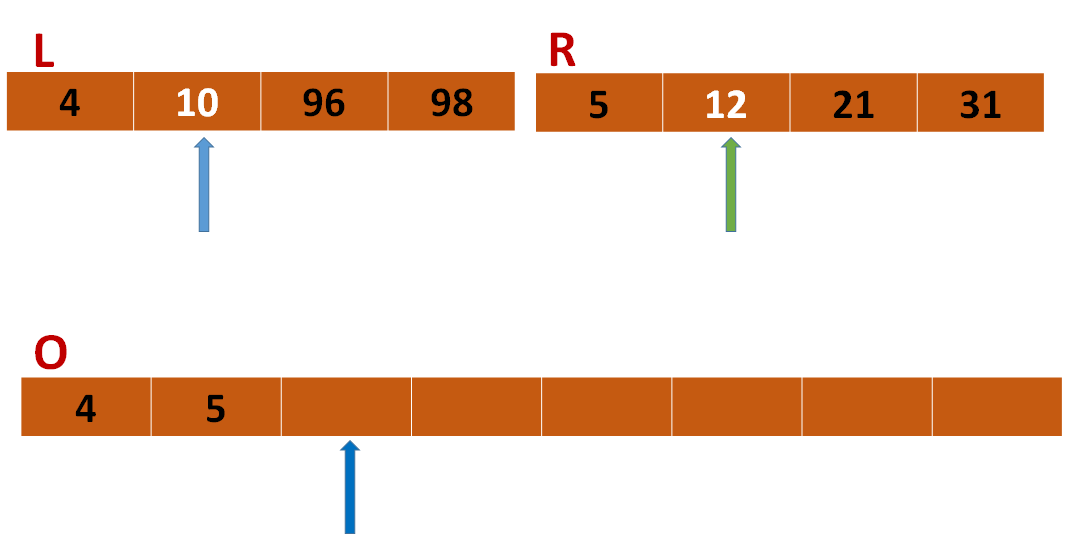
\includegraphics[scale=0.4]{mergeStep3.png}
\end{center}
\end{frame}




\begin{frame}{Merging Two Sorted Lists}
\begin{center}
    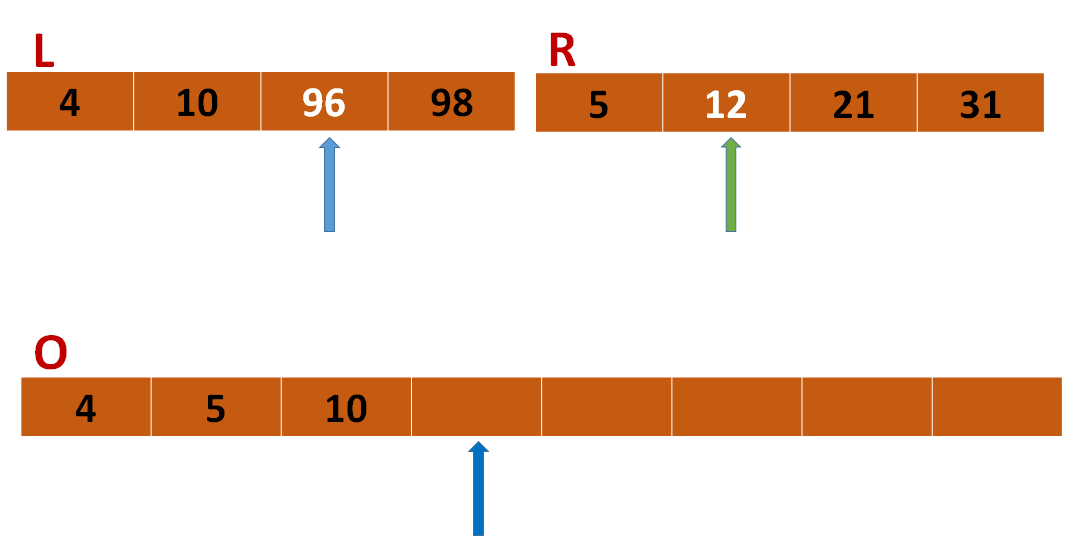
\includegraphics[scale=0.4]{mergeStep4.png}
\end{center}
\end{frame}




\begin{frame}{Merging Two Sorted Lists}
\begin{center}
    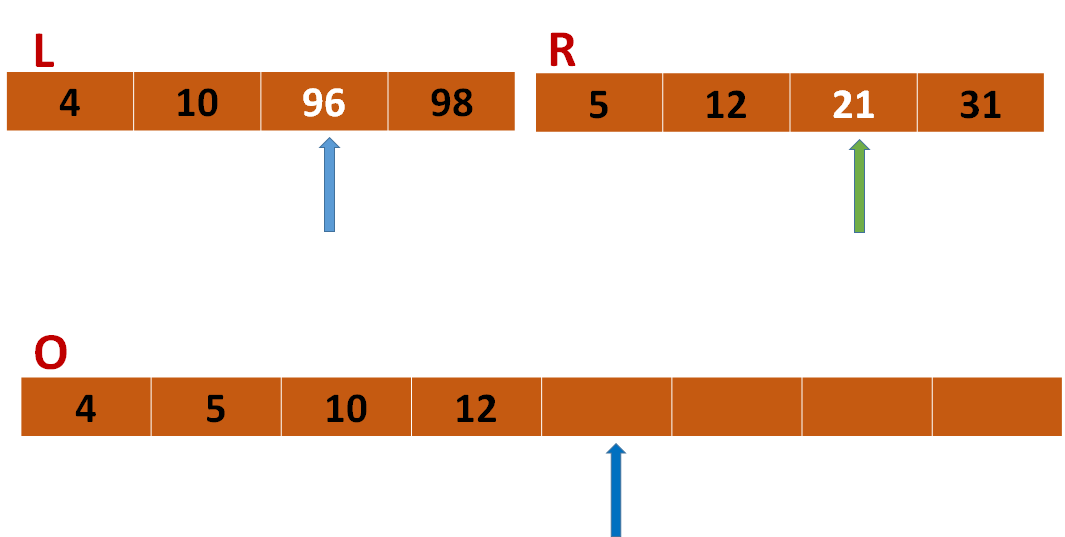
\includegraphics[scale=0.4]{mergeStep5.png}
\end{center}
\end{frame}




\begin{frame}{Merging Two Sorted Lists}
\begin{center}
    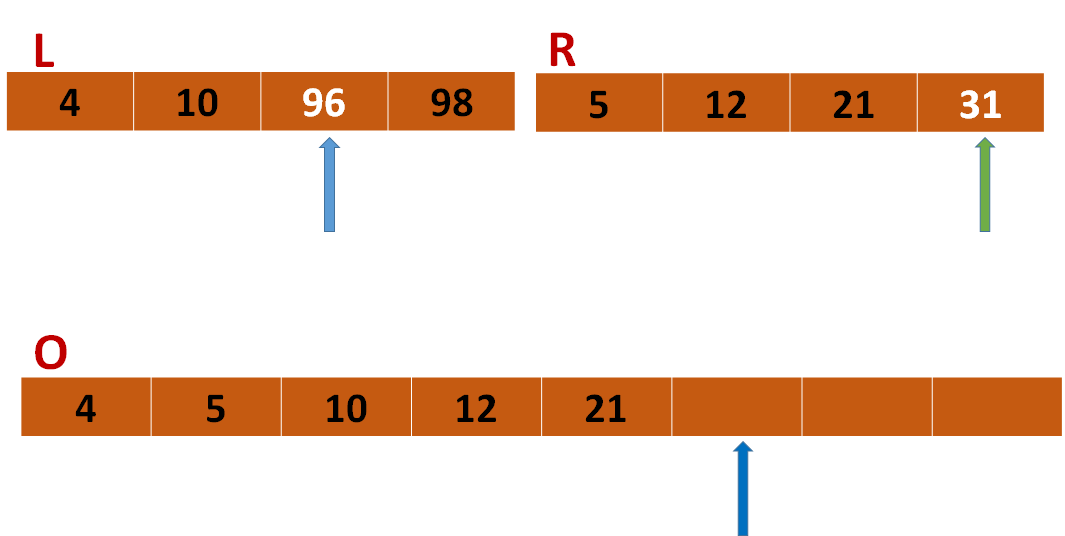
\includegraphics[scale=0.4]{mergeStep6.png}
\end{center}
\end{frame}




\begin{frame}{Merging Two Sorted Lists}
\begin{center}
    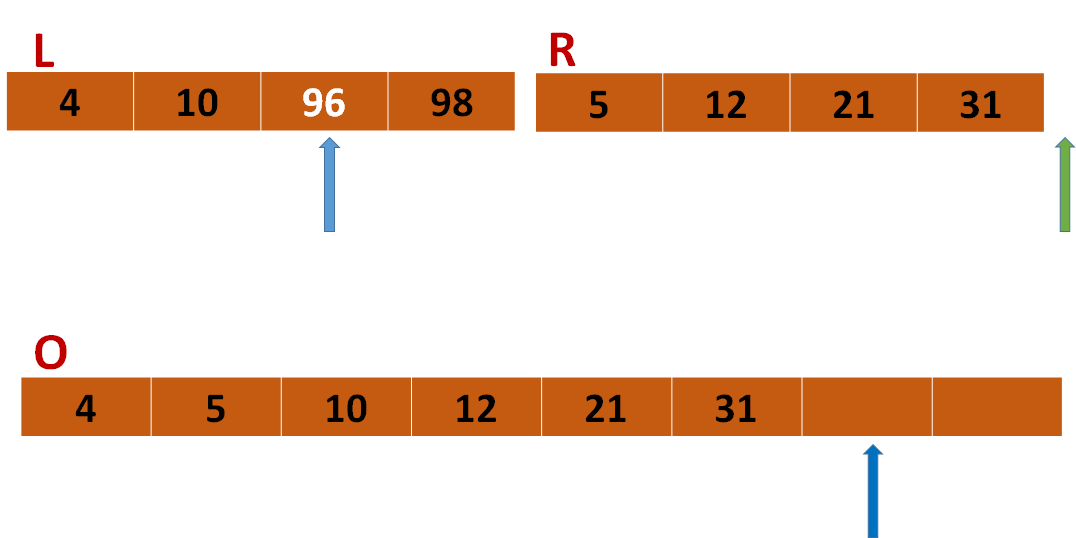
\includegraphics[scale=0.4]{mergeStep7.png}
\end{center}
\end{frame}




\begin{frame}{Merging Two Sorted Lists}
\begin{center}
    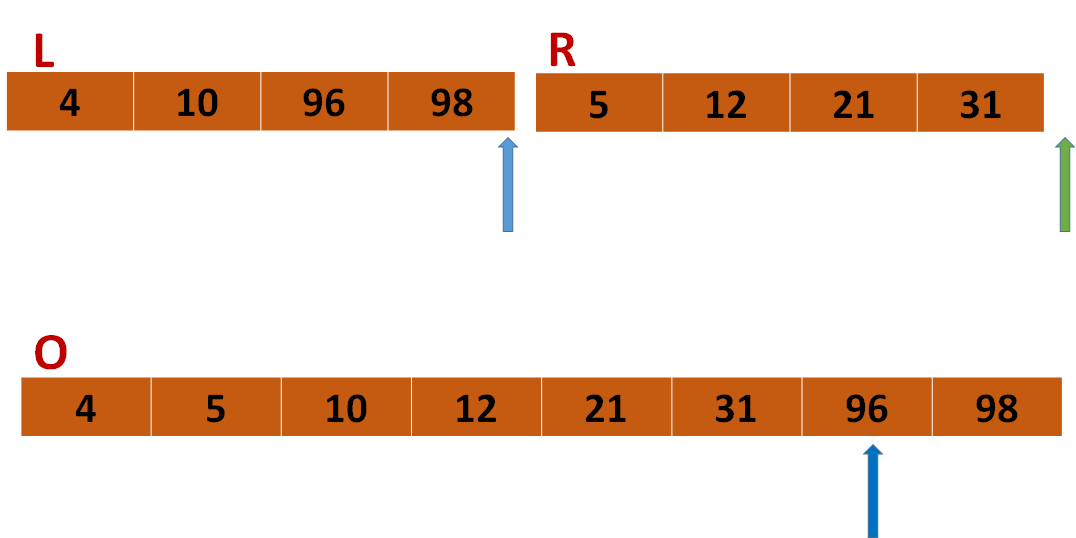
\includegraphics[scale=0.4]{mergeStep8.png}
\end{center}
\end{frame}


\begin{frame}[fragile]{Merging Two Sorted Lists}

\tblue{Merge Pseudocode:}

\begin{verbatim}
Merge(A,B,C):
    i = j = 1
    for k = 1 to n:
        if A[i] < B[j]:
            C[k] = A[i]
            i = i + 1
        else: (A[i] > B[j])
            C[k] = B[j]
            j = j + 1
\end{verbatim}
\end{frame}




\begin{frame}{Analyzing Merge Sort: Master Method}

\tblue{Quiz!}
\begin{itemize}
\item General recurrence formula for D\&C is  $T(n) = a T(\frac{n}{b}) + D(n) + C(n)$
\item What is $a$?
\item What is $b$?
\item What is $D(n)$?
\item What is $C(n)$?
\end{itemize}
\end{frame}


\begin{frame}{Analyzing Merge Sort: Master Method}

\tblue{Quiz!}
\begin{itemize}
\item General recurrence formula for D\&C is  $$T(n) = a T(\frac{n}{b}) + D(n) + C(n)$$
\item $a=2$, $b=2$
\item $D(n)=O(1)$
\item $C(n)=O(n)$
\item Combining, we get: $$T(n) = 2T(\frac{n}{2}) + O(n)$$
\item Using Master method, we get $T(n) = O(n \log n)$
\item If you are picky, $T(n) = T(\lceil \frac{n}{2} \rceil) + T(\lfloor \frac{n}{2} \rfloor) + O(n)$
\end{itemize}
\end{frame}


\begin{frame}{Analyzing Merge Sort: Recursion Tree\footnote{CLRS Book}}
\begin{center}
    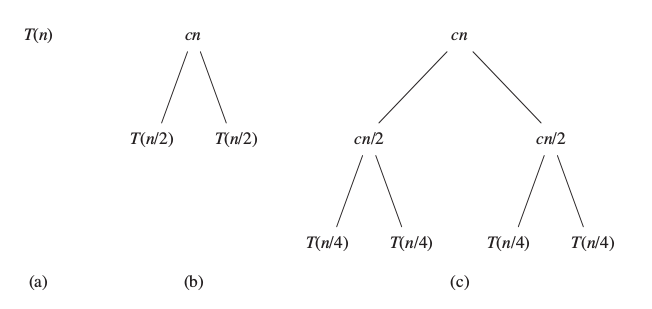
\includegraphics[scale=0.5]{mergeSortRecursionTree1.png}
\end{center}
\end{frame}



\begin{frame}{Analyzing Merge Sort: Recursion Tree\footnote{CLRS Book}}
\begin{center}
    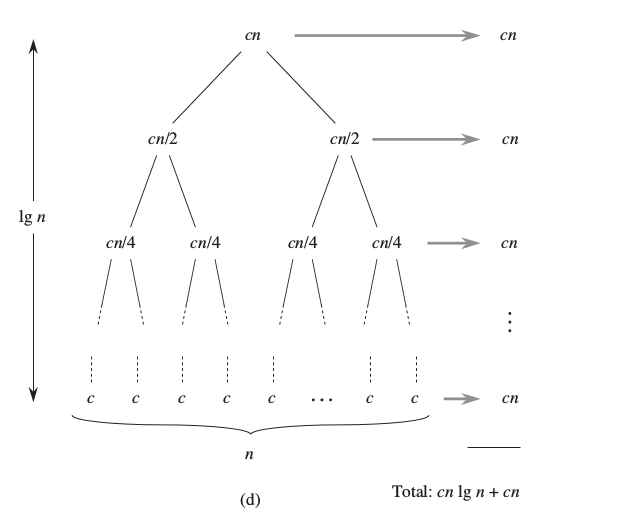
\includegraphics[scale=0.4]{mergeSortRecursionTree2.png}
\end{center}
\end{frame}


\begin{frame}{Merge Sort Vs Insertion Sort}
\begin{itemize}
\item Merge Sort is very fast in general ($O(n \log n)$) than Insertion sort ($O(n^2)$)
\item For ``nearly'' sorted arrays, Insertion sort is faster
\item Merge sort has $\hred{\Theta}(n \log n)$ (i.e. both best and worst case complexity is $n \log n$
\item Overhead: recursive calls and extra space for copying
\item Insertion sort is in-place and adaptive
\item Merge sort is easily parallizable 
\end{itemize}
\end{frame}

\begin{frame}{Quicksort}
\begin{itemize}
\item Quicksort is a {\em very} popular and elegant sorting algorithm
\item Invented by Tony Hoare
\begin{itemize}
    \item Also invented the concept of NULL (he called it a Billion dollar mistake! - why?)
    \item ``There are two ways of constructing a software design: One way is to make it so simple that there are obviously no deficiencies, and the other way is to make it so complicated that there are no obvious deficiencies. The first method is far more difficult.''
\end{itemize}
\end{itemize}
\end{frame}

\begin{frame}{Quicksort}
\begin{itemize}
\item Fastest of the fast sorting algorithms and lot (and lots) of ways to tune it.
\item Default sorting algorithm in most languages
\item Simple but innovative use of D\&C
\item On average it takes $\Theta(n \log n)$ but in worst case might require $O(n^2)$
\begin{itemize}
    \item Occurs rarely in practice {\bf if} coded properly
\end{itemize}
\end{itemize}
\end{frame}



\begin{frame}{Quicksort}
\begin{itemize}
\item Quicksort is a D\&C algorithm and uses a different style than Merge sort
\item It does more work in Divide phase and almost no work in Combine phase
\begin{itemize}
\item   One of the very few algorithms with this property
\end{itemize}
\end{itemize}
\end{frame}

\begin{frame}{Partitioning Choices\footnote{From \url{http://www.cs.bu.edu/fac/gkollios/cs113/Slides/quicksort.ppt}}}
\begin{itemize}
\item Sorting by D\&C - Divide to two sub-arrays, sort each and merge
\item Different partitioning ideas leads to different sorting algorithms
\item Given an array $A$ with $n$ elements, how to split to two sub-arrays $L$ and $R$ 
\begin{itemize}
    \item $L$ has first $n-1$ elements and $R$ has last element 
    \item $R$ has largest element of $A$ and $L$ has rest of $n-1$ elements
    \item $L$ has the first $\lfloor \frac{n}{2} \rfloor$ elements and $R$ has the rest
    \item Chose a pivot $p$, $L$ has elements less than $p$ and $R$ has elements greater than $p$
\end{itemize}
\end{itemize}
\end{frame}


\begin{frame}{Partitioning Choices}
\begin{itemize}
\item D\&C is not a silver bullet!
\item Different partitioning ideas leads to different sorting algorithms
\begin{itemize}
    \item {\bf Insertion Sort} $O(n^2)$: $L$ has first $n-1$ elements and $R$ has last element 
    \item {\bf Bubble Sort} $O(n^2)$: $R$ has largest element of $A$ and $L$ has rest of $n-1$ elements
    \item {\bf Merge Sort} $O(n \log n)$: $L$ has the first $\lfloor \frac{n}{2} \rfloor$ elements and $R$ has the rest
    \item {\bf Quick Sort} $O(n \log n)$ (average case): Chose a pivot $p$, $L$ has elements less than $p$ and $R$ has elements greater than $p$
\end{itemize}
\end{itemize}
\end{frame}

\begin{frame}[fragile]{Quicksort}

\tblue{Pseudocode:}
\begin{verbatim}
QuickSort(A, p, r):
    if p < r:
        q = Partition(A, p, r)
        QuickSort(A, p, q-1)
        QuickSort(A, q+1, r)
\end{verbatim}
\end{frame}



\begin{frame}{QuickSort}
\begin{center}
    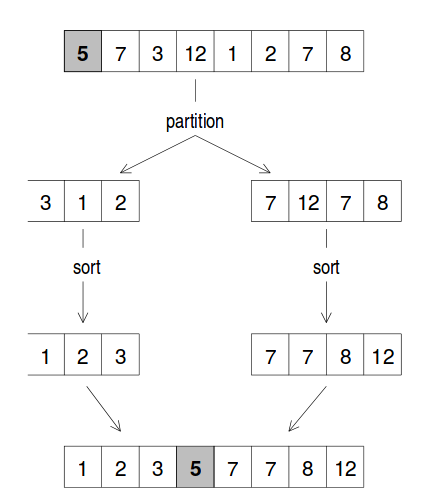
\includegraphics[scale=0.4]{quickSortHighLevelExample.png}
\end{center}
\end{frame}


\begin{frame}{Quicksort Design Objectives}
\begin{itemize}
\item Choose a good pivot
\item Do the partitioning - efficiently and in-place
\end{itemize}
\end{frame}


\begin{frame}{Partition Subroutine}
\begin{itemize}
\item Given a pivot, partition $A$ to two sub-arrays $L$ and $R$. 
\item All elements less then pivot are in $L$ 
\item All elements greater than pivot are in $R$
\item Return the new index of the pivot after the rearrangement
\item Note: Elements in $L$ and $R$ need not be sorted {\em during} partition (just $\leq$ pivot and $\geq$ pivot respectively)
\end{itemize}
\end{frame}


\begin{frame}{Partition Subroutine}
\begin{center}
    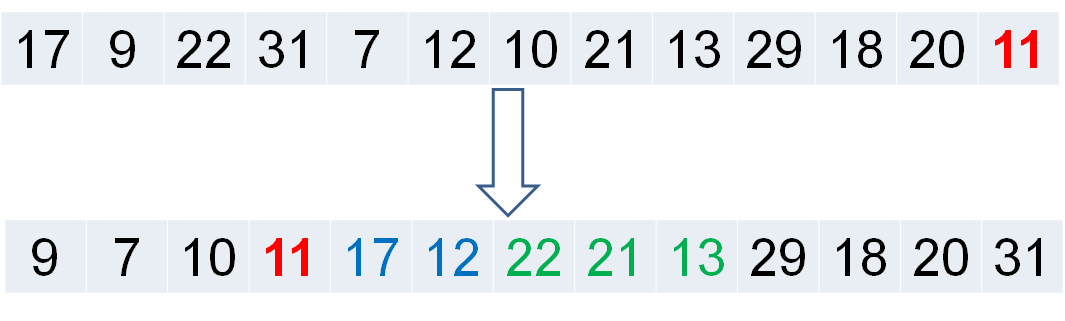
\includegraphics[scale=0.4]{partitionSubroutineMeta.png}
\end{center}
\end{frame}


\begin{frame}[fragile]{Partition Subroutine}

{\bf Note:} CLRS version of Partition subroutine. Assumes last element as pivot. 
To use this subroutine for other pivot picking strategies, swap pivot element with last element.

\begin{verbatim}
Partition(A, p, r):
    x = A[r] // x is the pivot
    i = p - 1
    for j = p to r-1
        if A[j] <= x 
            i = i + 1
            exchange A[i] with A[j]
    exchange A[i+1] with A[r]
    return i+1
\end{verbatim}
\end{frame}



\begin{frame}{Partition Example 1\footnote{\url{https://www.cs.rochester.edu/~gildea/csc282/slides/C07-quicksort.pdf}}}
\begin{center}
    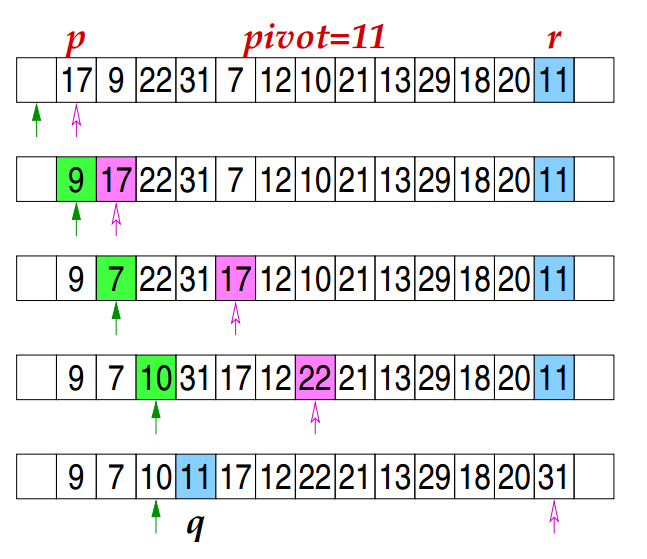
\includegraphics[scale=0.34]{partitionExample1.png}
\end{center}
\end{frame}


\begin{frame}{Partition Example 2\footnote{\url{https://www.cs.rochester.edu/~gildea/csc282/slides/C07-quicksort.pdf}}}
\begin{center}
    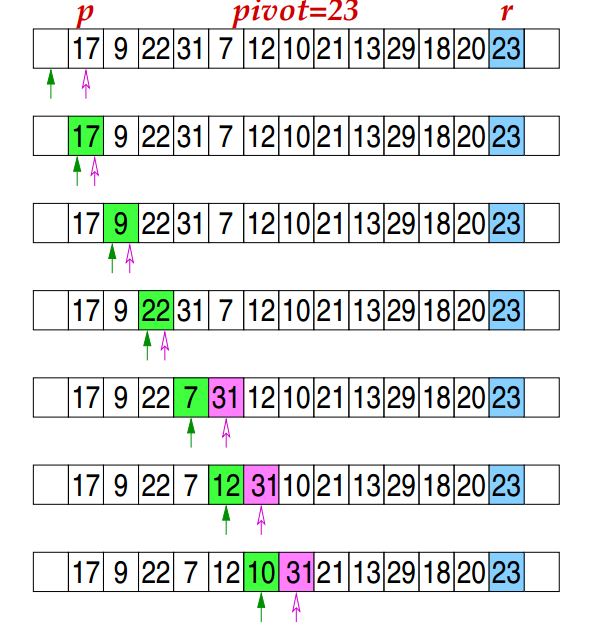
\includegraphics[scale=0.3]{partitionExample2.png}
\end{center}
\end{frame}


\begin{frame}{Partition Example 2\footnote{\url{https://www.cs.rochester.edu/~gildea/csc282/slides/C07-quicksort.pdf}}}
\begin{center}
    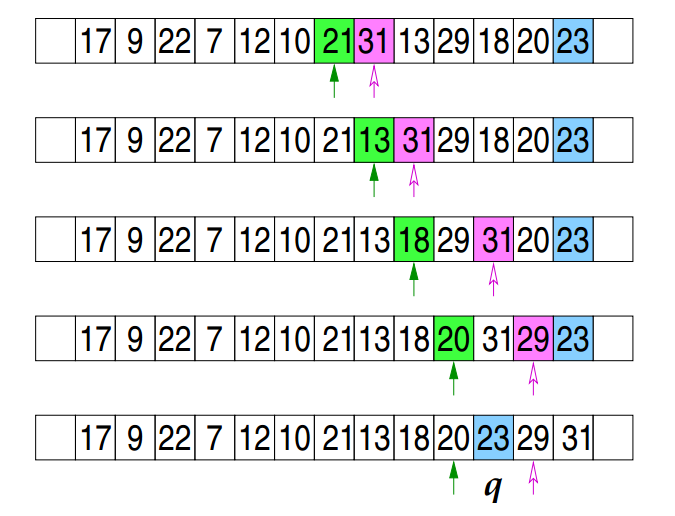
\includegraphics[scale=0.36]{partitionExample3.png}
\end{center}
\end{frame}



\begin{frame}{Partition Subroutine}
\begin{itemize}
\item Time Complexity: $O(n)$ - why?
\item Correctness: Why does it work?
\end{itemize}
\end{frame}


\begin{frame}{Quicksort: Best Case Scenario}
\begin{center}
    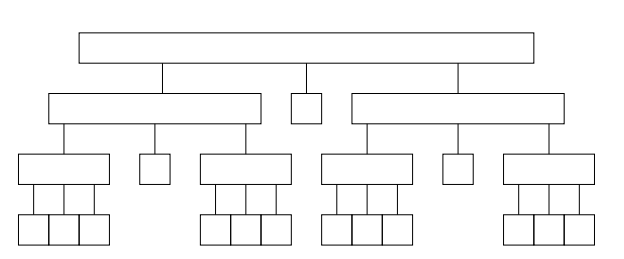
\includegraphics[scale=0.4]{quickSortBestCase.png}
\end{center}
\end{frame}


\begin{frame}{Quicksort: Worst Case Scenario}
\begin{center}
    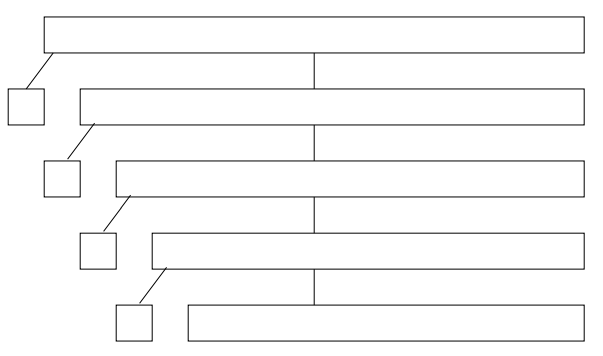
\includegraphics[scale=0.4]{quickSortWorstCase.png}
\end{center}
\end{frame}


\begin{frame}{Quicksort: Analysis}
Recurrence Relation for Quicksort:
\begin{itemize}
    \item Best Case: $T(n) = 2T(\frac{n}{2}) + n$ 
    \begin{itemize}
        \item Same as Merge sort: $\Theta(n \log n)$
    \end{itemize}
    \item Worst Case: $T(n) = T(n-1) + n$ 
    \begin{itemize}
        \item Same as Bubble sort: $O(n^2)$
    \end{itemize}
    \item Average Case: $T(n) = \sum_{p=1}^{n} \frac{1}{n} \left( T(p-1) + T(n-p) \right) + n$
    \begin{itemize}
        \item Analysis is very tricky, but returns $O(n \log n)$
        \item Intuition: Even an uneven split is okay (as long as it is between 25:75 to 75:25)
        \item When looking at all possible arrays of size $n$, we expect (on average) such a split to happen half the time 
    \end{itemize}

\end{itemize}
\end{frame}


\begin{frame}{Quicksort: Average Case Scenario}
\begin{center}
    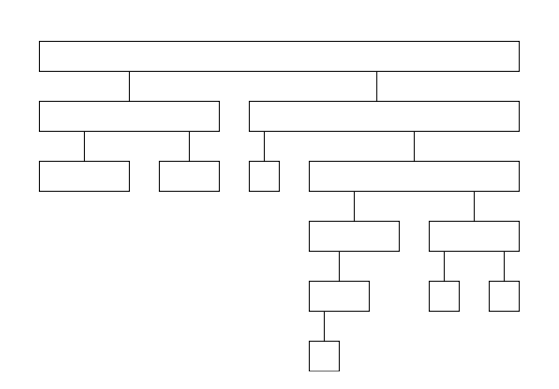
\includegraphics[scale=0.4]{quickSortAverageCase.png}
\end{center}
\end{frame}



\begin{frame}{Strategies to Pick Pivot}
\begin{itemize}
\item Pick first, middle or last element as pivot
\item Pick median-of-3 as pivot (i.e. median of first, middle and last element)
\item {\bf Bad News:} All of these strategies work well in practice, but has worst case time complexity of $O(n^2)$ 
\item Pick the median as pivot
\end{itemize}
\end{frame}



\begin{frame}[fragile]{Randomized Quicksort}
\begin{verbatim}
Randomized-Partition(A, p, r):
    i = Random(p,r)
    Exchange A[r] with A[i]
    return Partition(A, p, r)
\end{verbatim}

\begin{verbatim}
Randomized-QuickSort(A, p, r):
    if p < r:
        q = Randomized-Partition(A, p, r)
        Randomized-QuickSort(A, p, q-1)
        Randomized-QuickSort(A, q+1, r)
\end{verbatim}

\end{frame}



\begin{frame}{Randomized Quicksort}
\begin{itemize}
\item Adversarial analysis
\item It is easy to construct a worst case input for every deterministic pivot picking strategy 
\item Harder to do for randomized strategy
\item Idea: Pick a pivot randomly or shuffle data and use a deterministic strategy
\item {\em Expected} time complexity is $O(n \log n)$
\end{itemize}
\end{frame}


\begin{frame}{Sorting in the Real World}
\begin{itemize}
\item Sorting is a fundamental problem with intense ongoing research
\item No single best algorithm - Merge, Quick, Heap, Insertion sort all excel in some scenarions
\item Most programming languages implement sorting via tuned QuickSort (e.g. Java 6 or below) or 
a combination of Merge Sort and Insertion sort (Python, Java 7, Perl etc).
\end{itemize}
\end{frame}

\begin{frame}{Summary}

\tblue{Major Concepts:}
\begin{itemize}
\item D\&C - Divide, Conquer and Combine
\item Merge and Quick sort
\item Randomization as a strategy
\end{itemize}
\end{frame}


\end{document}

